\chapter{Modelled Systems}
\label{ch:modelledSystems}

The systems modelled in this thesis are exclusively systems which have closed form solutions when the Coulomb interaction is removed, i.e. in the non-interacting case. As discussed in Section \ref{sec:trialWF}, these closed form solutions are used to construct an optimal trial wave function in the form of a single Slater determinant. Without such an optimal basis, a single Slater determinant is not sufficient in Quantum Monte-Carlo (QMC) simulations. It is therefore not random that the focus of this thesis has been on various kinds of \textit{quantum dots} and \textit{atomic systems}, resembling the analytically solvable harmonic oscillator and the hydrogen atom respectively.

In this chapter atomic units will be used, that is, $\hbar=e=m_e=4\pi\epsilon_0 = 1$, where $m_e$ and $e_0$ is the electron mass and vacuum permittivity respectively.

\section{Atomic Systems}
\label{sec:modelAtoms}

Atomic systems are described as a number of electrons surrounding oppositely charged nuclei. As an approximation, the position of the nucleus is fixed. Due to the fact that the mass of the core is several orders of magnitude larger than the mass of the electrons, this serves as a very good approximation. In literature this is referred to as the \textit{Born-Oppenheimer Approximation} \cite{Sakurai:94}.

\subsection{The Single Particle Basis}

The single particle basis used to construct the trial wave functions for atomic systems originate from the closed form solutions for the hydrogen atom, i.e. one electron surrounding a single nucleus.

Given a nucleus with charge $Z$, the external potential between the electron and the core is

\begin{equation}
 \OP{v}_\mathrm{ext}(\mathbf{r}) = -\frac{Z}{r}, \label{eq:v0hydro}
\end{equation}

\begin{figure}
 \begin{center}
  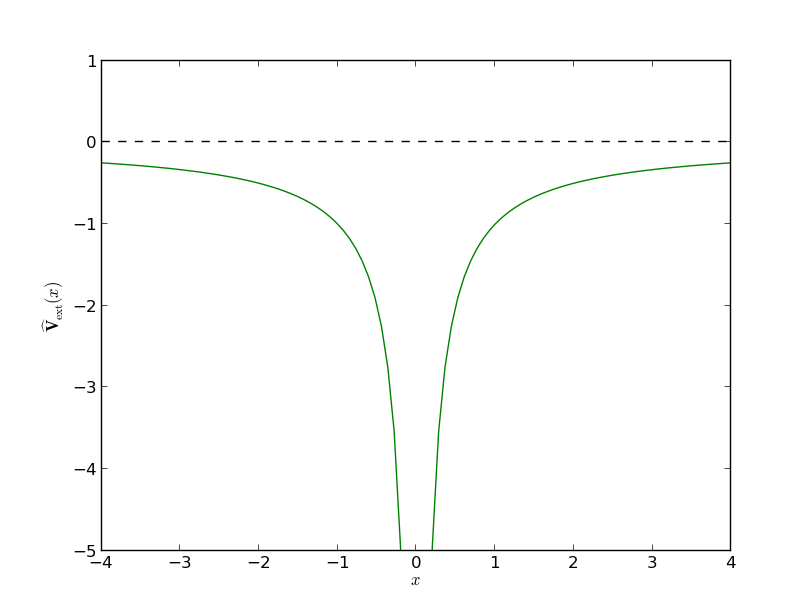
\includegraphics[scale=0.5]{../Graphics/Potentials/hydrogen.png}
  \caption{The one dimensional version of the single particle potential of hydrogen from Eq.~(\ref{eq:v0hydro}). The potential is spherically symmetric for three dimensions and can be visualized by rotating the figure around all axes. The potential has a strong singularity at the origin, which originates from the fact that the nucleus (located at the origin) and the electrons have opposite charges, that is, they feel an attractive force.}
  \label{fig:extPotHydrogen}
 \end{center}
\end{figure}

which results in the following single particle Hamiltonian:

\begin{equation}
 \OP{h}_0(\mathbf{r}) = -\frac{1}{2}\nabla^2 - \frac{Z}{r}.
\end{equation}

The external potential is displayed in figure \ref{fig:extPotHydrogen}. The eigenfunctions of the Hamiltonian are \cite{griffiths}

\begin{equation}
 \phi_{nlm}(r, \theta, \phi; Z) \propto r^l e^{-Zr/n}\left[L_{n-l-1}^{2l+1}\left(\frac{2r}{n}Z\right)\right] Y_l^m(\theta, \phi), \label{eq:hydrogenBasisComplex}
\end{equation}

where $L_{q-p}^p(x)$ are the \textit{associated Laguerre polynomials} and $Y_l^m(\theta, \phi)$ are the \textit{spherical harmonics}. The spherical harmonics are related to the \textit{associated Legendre functions} $P_l^m$ in the following manner:

\begin{equation}
 Y_l^m(\theta, \phi) \propto   P_l^m(\cos\theta)e^{im\phi}, \label{eq:spherHarm}
\end{equation}

In the current model, the principal quantum number $n$ together with $Z$ control the energy level of the atom, 

\begin{equation}
 E(n; Z) = -\frac{Z^2}{2n^2}\label{eq:AtomNonIntEnergy}
\end{equation}

which implies that the energy levels are degenerate for all combinations of $l$ and $m$. For a given value of $n$, the allowed levels of the \textit{azimuthal} quantum number $l$ and the \textit{magnetic} quantum number $m$ is 

\begin{align*}
 n &= 1, 2, ... \\
 l &= 0, 1, ...\,, n-1 \\
 m &= -l, -l + 1, ...\,, l - 1, l
\end{align*}


which defines the shell structure of the hydrogen atom. 

A problem with the single particle basis of hydrogen is the complex terms in Eq.~(\ref{eq:spherHarm}), i.e. the spherical harmonics. Complex bases will require the entire code to work with complex variables, which should be avoided if possible. For this reason, the spherical harmonics in Eq.~(\ref{eq:hydrogenBasisComplex}) are substituted with the real-valued \textit{solid harmonics} $S_l^m(r, \theta, \phi)$  \cite{SolidHarmonics}

\begin{align}
S_l^m(r, \theta, \phi) &= (-1)^m\frac{(1+m)!}{2}r^l\left[Y_l^m(\theta, \phi) + (-1)^m Y_l^{-m}(\theta, \phi)\right] \\
 &= (-1)^m r^{l} P_l^{|m|}(\cos\theta) \begin{cases} \cos m\phi & m \ge 0 \\ \sin|m|\phi &  m < 0 \end{cases},                                                                                                     
\end{align}

which results in the following real eigenfunctions

\begin{equation}
  \phi_{nlm}(r, \theta, \phi; k) \propto e^{-kr/n}\left[L_{n-l-1}^{2l+1}\left(\frac{2r}{n}k\right)\right] S_l^m(r, \theta, \phi) \equiv \phi^\mathrm{H}_{nlm}(\mathbf{r}), \label{eq:hydrogenBasisReal}
\end{equation}

where $k = \alpha Z$ is a scaled charge with $\alpha$ as a variational parameter chosen by methods described in Section \ref{sec:selectingOptVarPar}.

A set of quantum numbers $nlm$ is mapped to a single index $i$. A listing of all the single particle wave functions and their closed form derivatives are given in Appendix \ref{appendix:SymPyHydro}.

\subsection{Atoms}

An atom is described as $N$ electrons surrounding a fixed nucleus of charge $Z=N$. The Hamiltonian consists of $N$ single particle hydrogen Hamiltonians in addition to the Coulomb interaction, which results in

\begin{align}
 \OP{H}_{\mathrm{Atoms}}(\mathbf{r}) &= \sum_{i=1}^N \OP{h}_0(\mathbf{r}_i) + \sum_{i<j} \frac{1}{r_{ij}} \\
                         &= \sum_{i=1}^N \left[-\frac{1}{2}\nabla_i^2 - \frac{Z}{r_i}\right] + \sum_{i<j} \frac{1}{r_{ij}},
\end{align}

where $r_{ij} = |\mathbf{r}_i -\mathbf{r}_j|$. Excluding the Coulomb term, the Hamiltonian can be decoupled into single particle terms with a total ground state energy

\begin{equation}
 E_0 = -\frac{Z^2}{2}\sum_{i=1}^N \frac{1}{n_i^2}. \label{eq:atomsE0}
\end{equation}

The Slater determinant is set up to fill the $N$ lowest lying states, that is, the $N$ states with lowest $n$ without breaking the Pauli principle, using the single particle orbitals from Eq.~(\ref{eq:hydrogenBasisReal}). The degeneracy of level $n$ in an atom is given by the following expression:

\begin{equation}
g(n) = 2\sum_{l=0}^{n-1}\sum_{m={-l}}^l 1 = 2n^2. 
\end{equation}

\subsection{Homonuclear Diatomic Molecules}
\label{sec:homoMolecules}

A homonuclear diatomic molecule consists of two atoms (diatomic molecule) of the same element (homonuclear) with charge $Z=N/2$, separated by a distance $R$. The origin is set between the atoms, which are fixed at positions $\pm \mathbf{R}/2$. An electron at position $\mathbf{r}_i$ gets a contribution from both the cores as displayed in figure \ref{fig:dimolecules}. In addition, there is a repulsive Coulomb potential between the two cores equal to $Z^2/R$. The resulting Hamiltonian becomes

\begin{equation}
 \OP{H}_{\mathrm{Mol.}}(\mathbf{r}, \mathbf{R}) = \sum_{i=1}^N \left[-\frac{1}{2}\nabla_i^2 + \frac{Z}{|\mathbf{r}_i + \mathbf{R}/2|} + \frac{Z}{|\mathbf{r}_i - \mathbf{R}/2|}\right] + \frac{Z^2}{R} + \sum_{i<j} \frac{1}{r_{ij}}.
\end{equation}



\begin{figure}
 \begin{center}
  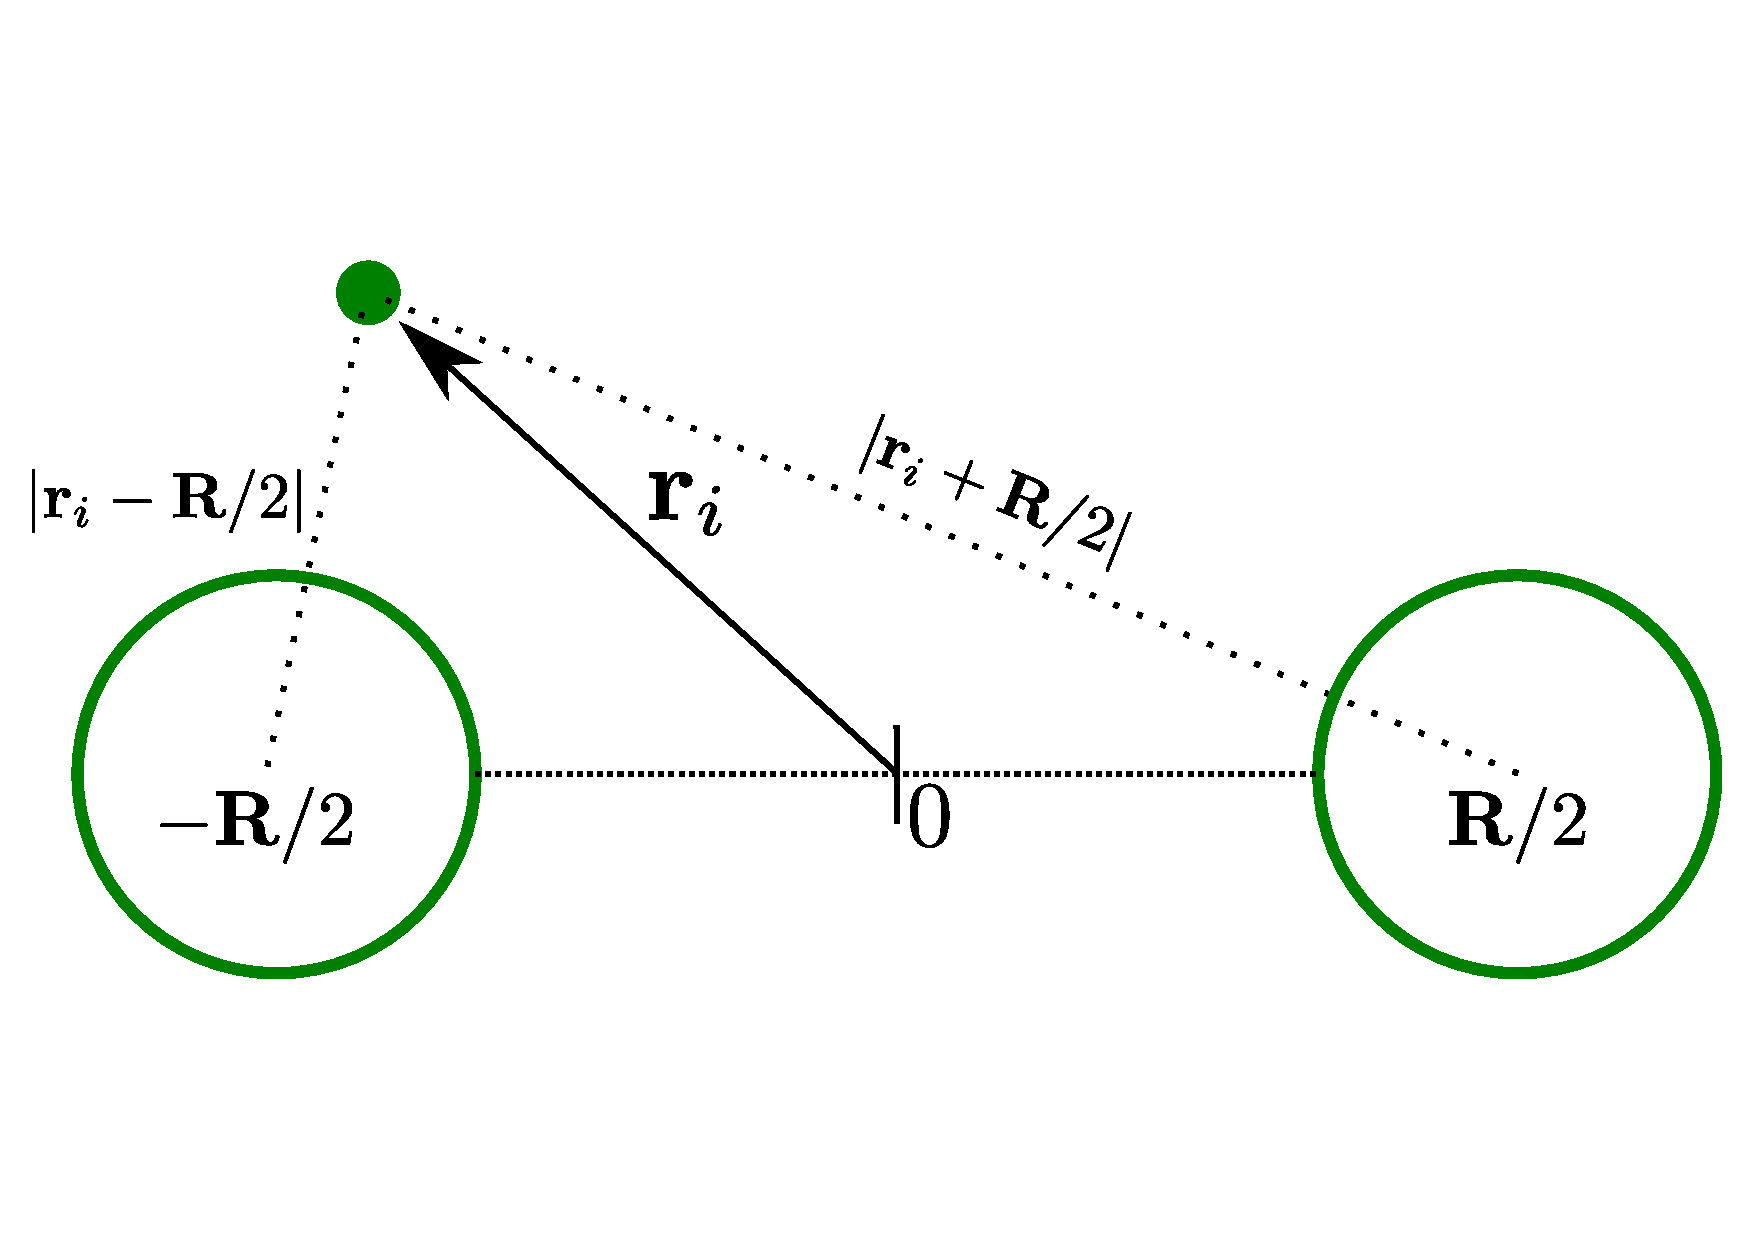
\includegraphics[scale=0.3]{../Graphics/Molecules.pdf}
  \caption{The model for the diatomic molecule used in this thesis. The two largest circles represents the atoms. An electron at position $\mathbf{r}_i$ gets a potential energy contribution from both the cores equal to $Z/|\mathbf{r}_i + \mathbf{R}/2|$ and  $Z/|\mathbf{r}_i - \mathbf{R}/2|$, where Z is the charge of the nuclei (homonuclear). The diatomic molecular wave functions are set up as a superposition of two hydrogen-like wave functions, one at position $\mathbf{r}_i + \mathbf{R}/2$ and the second at position $\mathbf{r}_i - \mathbf{R}/2$.}
  \label{fig:dimolecules}
 \end{center}
\end{figure}


In order to transform the hydrogen eigenstates $\phi_{nlm}^\mathrm{H}(\mathbf{r})$, which are symmetric around a single nucleus, into molecular single particle states $\phi_{nlm}^\pm (\mathbf{r}_i)$, a superposition of the two mono-nucleus wave functions are used

\begin{align}
 \phi_{nlm}^+ (\mathbf{r}_i, \mathbf{R}) &= \phi_{nlm}^\mathrm{H}(\mathbf{r}_i + \mathbf{R}/2) + \phi_{nlm}^\mathrm{H}(\mathbf{r}_i - \mathbf{R}/2)\label{eq:moleculeTransPlus}, \\
 \phi_{nlm}^- (\mathbf{r}_i, \mathbf{R}) &= \phi_{nlm}^\mathrm{H}(\mathbf{r}_i + \mathbf{R}/2) - \phi_{nlm}^\mathrm{H}(\mathbf{r}_i - \mathbf{R}/2)\label{eq:moleculeTransMin},
\end{align}

which reads ``electron surrounding first nucleus combined with electron surrounding second nucleus''. See figure \ref{fig:dimolecules} for a better view. 

As seen from the equations above, there are necessarily two ways of doing this superposition: Adding and subtracting the states. It is easy to show that 

\begin{equation}
 \braket{\phi_{n'l'm'}^-}{\phi_{nlm}^+} = 0,
\end{equation}

which implies that these states form an expanded complete set of single particle states for the molecular system, resulting in a four-fold degeneracy in each set of quantum numbers $nlm$. It is necessary to use both the positive and negative states in order to fit e.g. four electrons into $n=0$ for the case of the lithium molecule ($N=6$). Using only the positive or only the negative states would result in a singular Slater determinant.

Using $\mathbf{R} = \left(R_x, R_y, R_z\right)$ as the vector separating the atoms, $\mathbf{j} = (0, 1, 0)$ as the unit vector in the $y$-direction, $\mathbf{r}_i = \left(x_i, y_i, z_i\right)$ as the electron position, and the chain rule of derivation, the gradient in the $\mathbf{j}$-direction becomes

\begin{align}
 \mathbf{j}\cdot \nabla_i \phi_{nlm}^\pm (\mathbf{r}_i, \mathbf{R}) &= \underbrace{\frac{\partial (y_i + R_y/2)}{\partial y_i}}_{1}\frac{\partial \phi_{nlm}^\mathrm{H}(\mathbf{r}_i + \mathbf{R}/2)}{\partial (y_i + R_y/2)} \notag \\
  &\pm \underbrace{\frac{\partial (y_i - R_y/2)}{\partial y_i}}_{1}\frac{\partial \phi_{nlm}^\mathrm{H}(\mathbf{r}_i - \mathbf{R}/2)}{\partial (y_i - R_y/2)} \notag\\
  &= \frac{\partial \phi_{nlm}^\mathrm{H}(\mathbf{r}_i + \mathbf{R}/2)}{\partial (y_i + R_y/2)} \pm \frac{\partial \phi_{nlm}^\mathrm{H}(\mathbf{r}_i - \mathbf{R}/2)}{\partial (y_i - R_y/2)} \notag\\
  &=  \frac{\partial \phi_{nlm}^\mathrm{H}(\mathbf{\tilde R_i^+})}{\partial \tilde Y_i^+} \pm \frac{\partial \phi_{nlm}^\mathrm{H}(\mathbf{\tilde R_i^-})}{\partial \tilde Y_i^-}, \label{eq:MoleculeWorksWithOldFunctions}
\end{align}

where $\mathbf{\tilde R_i^\pm} = \mathbf{r}_i \pm \mathbf{R}/2 = (\tilde X_i^\pm, \tilde Y_i^\pm, \tilde Z_i^\pm)$ represents the electron position in the reference frame of the two nuclei. Equation (\ref{eq:MoleculeWorksWithOldFunctions}) demonstrates that the closed form expressions used in simulations of single atoms can be reused in the case of diatomic molecules. In other words, the functions in Appendix \ref{appendix:SymPyHydro} can simply be called  with $\mathbf{\tilde R_i^\pm}$ instead of $\mathbf{r}_i$ and then be either subtracted or added. This result holds for the Laplacian as well.

The non-interacting energy is equal to that of the regular atoms in the limit $R\to\infty$, however, now with a four-fold degeneracy and a charge equal to $N/2$. This four-foulding also implies that the degeneracy of level $n$ becomes $g(n) = 4n^2$.

\section{Quantum Dots}
\label{sec:modelQDots}

Quantum dots are electrons confined within a potential well. This potential well can be broadened and narrowed in such a way that the material properties of the quantum dot can be tuned to desired values. Such manufactured quantum dots have practical applications in solar cells \cite{QDOTS_SOLAR}, lasers \cite{QDOTS_LASER}, medical imaging \cite{QDOTS_MEDICINE}, and quantum computing \cite{QDOTS_QUANTUM}, however, the focus on quantum dots in this thesis has been purely academic.

Understanding the physics behind strongly and weakly confined electrons are of great importance when it comes to understanding many-body theory in general. The purpose of studying quantum dots from an academic point of view is to investigate the behavior of the system a function of the level of confinement and the number of electrons.

The model for the quantum dot used in this thesis is electrons trapped in a harmonic potential with frequency $\omega$, which in the case of no Coulomb interaction can be solved analytically. 

\subsection{The Single Particle Basis}

Just as the hydrogen potential was used to describe atoms, the \textit{harmonic oscillator} potential is used as the single particle Hamiltonian describing quantum dots, that is, an external one-body potential on the form 

\begin{equation}
 \OP{v}_\mathrm{ext}(\mathbf{r)} = \frac{1}{2}\omega^2r^2,
\end{equation}

\begin{figure}
 \begin{center}
  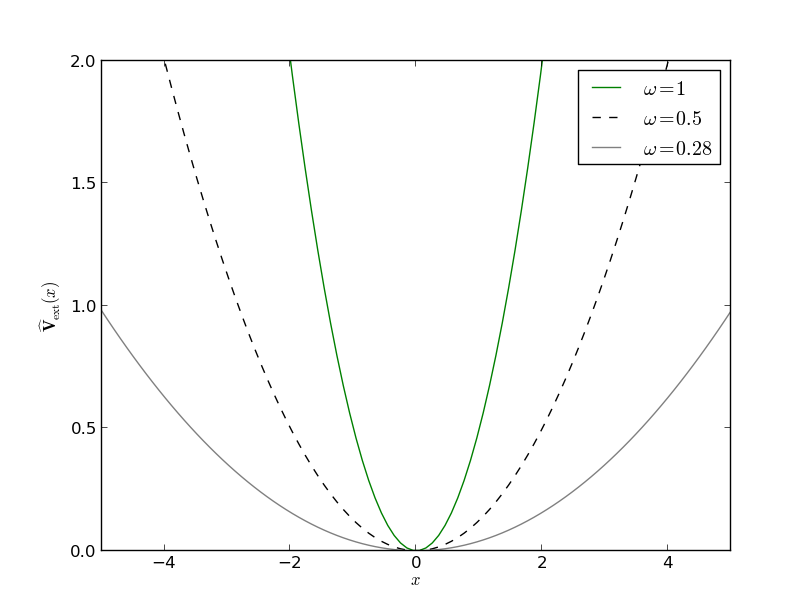
\includegraphics[scale=0.5]{../Graphics/Potentials/qdots.png}
  \caption{A one dimensional version of the single particle potential of quantum dots. In two - and three dimensions, the potential is rotationally/spherically symmetric and equal along all axes. Just as the hydrogen potential in figure \ref{fig:extPotHydrogen}, the electrons are drawn to the center.}
  \label{fig:extPotQDOTS}
 \end{center}
\end{figure}

where $\omega$ is the oscillator frequency representing the strength for the confinement. The potential for different $\omega$ is presented in figure \ref{fig:extPotQDOTS}. The single particle Hamiltonian is thus

\begin{equation}
 \OP{h}_0(\mathbf{r}) = -\frac{1}{2}\nabla^2 + \frac{1}{2}\omega^2r^2.
\end{equation}

The eigenfunctions of the Hamiltonian for two and three dimensions are \cite{Sakurai:94}

\begin{align}
\phi_{n_x, n_y}(\mathbf{r}) &= H_{n_x}(\sqrt{w}x)H_{n_y}(\sqrt{w}y)e^{-\frac{1}{2}wr^2} \\
\phi_{n_x, n_y, n_z}(\mathbf{r}) &= H_{n_x}(\sqrt{w}x)H_{n_y}(\sqrt{w}y)H_{n_z}(\sqrt{w}z)e^{-\frac{1}{2}wr^2},
\end{align}

where $H_n(x)$ is the $n$'th level Hermite polynomial. The shell structures in quantum dots arise from different combinations of $n_x$, $n_y$, and for three dimensions $n_z$, which sums up to the same $n$.

The variational parameter $\alpha$ is introduced by letting $\omega\to\alpha\omega$, just as $Z\to\alpha Z$ for atoms. Defining $k\equiv\sqrt{\alpha\omega}$, the eigenfunctions which are used as the single particle orbitals for quantum dots in this thesis are

\begin{align}
\phi_{n_x, n_y}(\mathbf{r}) &= H_{n_x}(kx)H_{n_y}(ky)e^{-\frac{1}{2}k^2r^2}, \\
\phi_{n_x, n_y, n_z}(\mathbf{r}) &= H_{n_x}(kx)H_{n_y}(ky)H_{n_z}(kz)e^{-\frac{1}{2}k^2r^2}.
\end{align}

As for the hydrogen states, a set of quantum numbers are mapped to an integer $i$.  A listing of all the single particle wave functions and their closed form derivatives are given in Appendix \ref{appendix:SymPyHO} for two dimensions and Appendix \ref{appendix:SymPyHO3D} for three dimensions. 


\subsection{Two - and Three Dimensional Quantum Dots}

A quantum dot is described as $N$ electrons confined in an oscillator potential with frequency $\omega$. The Hamiltonian is

\begin{align}
 \OP{H}_{\mathrm{Q.D.}}(\mathbf{r}) &= \sum_{i=1}^N \OP{h}_0(\mathbf{r}_i) + \sum_{i<j} \frac{1}{r_{ij}} \\
                         &= \sum_{i=1}^N \left[-\frac{1}{2}\nabla_i^2 + \frac{1}{2}\omega^2r_i^2 \right] + \sum_{i<j} \frac{1}{r_{ij}},
\end{align}

where $r_{ij} = |\mathbf{r}_i -\mathbf{r}_j|$. Excluding the Coulomb term, the Hamiltonian can be decoupled into single particle terms with a total ground state energy \cite{griffiths}

\begin{equation}
 E_0 = \omega\sum_{i=1}^N \left(n_i + \frac{d}{2}\right), \label{eq:qdotsE0}
\end{equation}

where $d$ is the number of dimensions, $n_i = n_x + n_y + n_z \ge 0$ for three dimensions and $n_i = n_x + n_y \ge 0$ for two dimensions. The degeneracy of level $n$ in a quantum dot is $g(n) = 2n$ for two dimensions and $g(n) = (n+2)(n+1)$ for three dimensions.

The Slater determinant is set up to fill the $N$ lowest lying states, that is, the $N$ states with lowest $n$ without breaking the Pauli principle, using the single particle orbitals from Eq.~(\ref{eq:hydrogenBasisReal}).


\subsection{Double-well Quantum Dots}

The same strategy used to transform an atomic system into a homonuclear diatomic molecular system can be applied to two dimensional quantum dots, resulting in a double-well quantum dot. Double-well quantum dots are used as a practical quantum dot system in experiments \cite{doubleWellExpt}. 

The model for the double-well potential used in this thesis is \cite{ymwang}

\begin{equation}
 \OP{v}_{ext}(\mathbf{r}) = \frac{1}{2}m^\ast \omega_0^2 \left[r^2 + \frac{1}{4}R^2 - R|x|\right], \label{eq:VextDoubleWell}
\end{equation}

where $R$ is the distance between the wells, $m^\ast$ is a material parameter and $\omega_0$ is the confinement strength. For simplicity, the wells are separated in the $x$-direction. The potential is presented in figure \ref{fig:extPotDoubleWell}.

\begin{figure}
 \begin{center}
  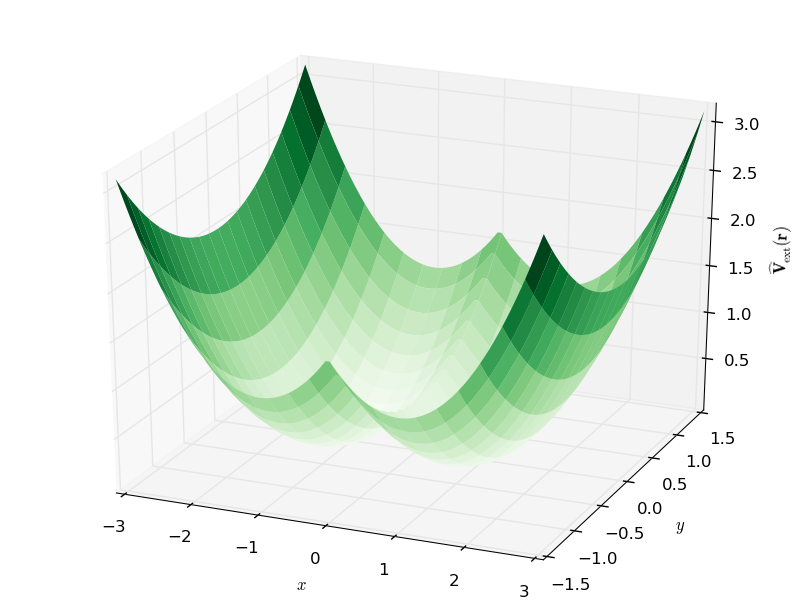
\includegraphics[scale=0.5]{../Graphics/Potentials/doubleWell.png}
  \caption{The external potential for a double-well quantum dot from Eq.~(\ref{eq:VextDoubleWell})} with $R=2$ and $m^\ast\omega_0^2 = 1$, where $R$ is the distance between the well centers and $m^\ast$ and $\omega_0$ are material constants.  
  \label{fig:extPotDoubleWell}
 \end{center}
\end{figure}

The full Hamiltonian becomes

\begin{equation}
  \OP{H}_{\mathrm{QDDW}}(\mathbf{r}, \mathbf{R}) = \sum_{i=1}^N \left(-\frac{1}{2m^\ast}\nabla_i^2 + \frac{1}{2}m^\ast \omega_0^2 \left[r^2 + \frac{1}{4}R^2 - R|x_i|\right]  \right) + \sum_{i<j} \frac{1}{r_{ij}},
\end{equation}

which can be simplified to fit the standard form of the previous Hamiltonians by letting $r_i\to\sqrt{m^\ast}r_i$. Applying this transformation of coordinates yields

\begin{align}
  \OP{H}_{\mathrm{QDDW}}(\mathbf{r}, \mathbf{R}) &\to \OP{H}_{\mathrm{QDDW}}(\sqrt{m^\ast}\mathbf{r}, \sqrt{m^\ast}\mathbf{R}) \\
   &=\sum_{i=1}^N \left(-\frac{1}{2}\nabla_i^2 + \frac{1}{2} \omega_0^2 \left[r^2 + \frac{1}{4}R^2 - R|x_i|\right]  \right) + \sqrt{m^\ast}\sum_{i<j} \frac{1}{r_{ij}}.
\end{align}

The eigenstates are, as for the homonuclear diatomic molecules in Eq.~(\ref{eq:moleculeTransPlus}) and (\ref{eq:moleculeTransMin}), given as positive and negative superpositions of the standard harmonic oscillator eigenstates. As shown for molecules in Eq.~(\ref{eq:MoleculeWorksWithOldFunctions}), the closed form expressions for the single-well quantum dot can be reused in the case of a double-well quantum dot. 

The degeneracy of the $n$'th level is $g(n) = 4n$. The non-interacting single particle energies are identical to those of the single-well in the limit $R\to\infty$, that is, in the case of two decoupled potential wells.

